This example shows a trick to realize a target with two planar crystalline
layers by connecting the two layers outside the implantation area in a 2-D
setup.

The input file reads:

\begin{verbatim}
B implantation in a multilayer structure using the "2D trick"
B 30 keV, 7 tilt, a/c/a/c
 &setup    ndim=2 natom=3 nr=3 nion=50000 nionhis=800 /
 &ions     name='B' energy=30 dose=5.E13 tilt=7. rotate=15. diverg=0.3 /
 &material region=1 name='SiO2' xtal='no' /
 &material region=2 name='Si' xtal='yes' wafer=0.,0.,1. vsurf=1.,1.,0. /
 &material region=3 name='SiO2' xtal='no' /
 &geometry point=1 pos=-3000,0 /
 &geometry point=2 pos=-3000,80 /
 &geometry point=3 pos=-3000,3000 /
 &geometry point=4 pos=3000,3000 /
 &geometry point=5 pos=3000,480 /
 &geometry point=6 pos=-2900,480 /
 &geometry point=7 pos=-2900,380 /
 &geometry point=8 pos=3000,380 /
 &geometry point=9 pos=3000,80 /
 &geometry point=10 pos=3000,0 /
 &geometry region=1 points=1,2,9,10 /
 &geometry region=2 points=2,3,4,5,6,7,8,9 /
 &geometry region=3 points=7,6,5,8 /
 &output   lmom=t lhis=t lhis2=t /
\end{verbatim}

\begin{figure}[htbp]
\centering
\noindent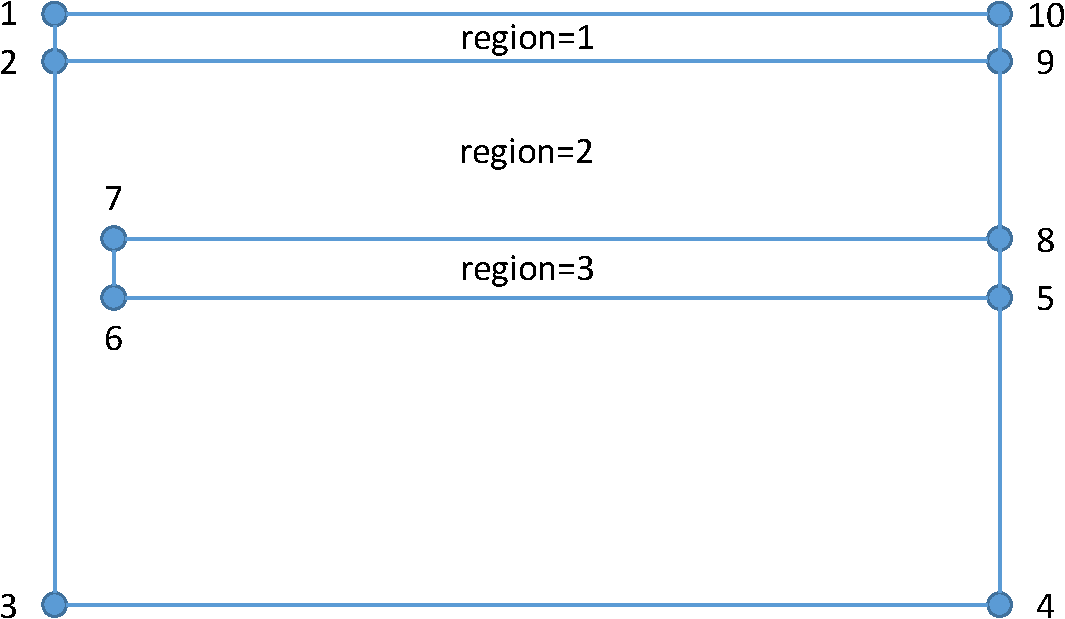
\includegraphics[scale=0.6]{ex_multilayer-crop.pdf}
\caption{Geometry of the multilayer example. Lengths are not to scale. The
point and region indices are indicated.}
\label{fig:multilayer}
\end{figure}

Here, three regions are defined (\texttt{nr=3} on the \texttt{\&SETUP} record,
three \texttt{\&MATERIAL} and four \texttt{\&GEOMETRY} records). The geometry
defined by the input file is visualized in Fig.~\ref{fig:multilayer}. Since
\texttt{xinit} is not specified on the \texttt{\&IONS} record, its default
value 0 is used. That means, all ions are implanted in the center of the target
at $x=0$, and their lateral straggle will not suffice for them to reach beyond
points 6 and 7 laterally.

In the definition of the material of region 2, the orientation of the crystal
with respect to the $x$ and $z$ axes is specified: The $z$ axis is parallel to
the [001] direction (\texttt{wafer=0.,0.,1.}), and the $x$ axis is parallel to
[110] (\texttt{vsurf=1.,1.,0.}).

